\documentclass[11pt]{article}
\usepackage[margin=1.1in]{geometry}
\usepackage{amsmath, amssymb, amsthm}
\usepackage{booktabs}
\usepackage{graphicx}
\usepackage{listings}
\usepackage{xcolor}
\usepackage{hyperref}
\hypersetup{colorlinks=true, linkcolor=blue!50!black, urlcolor=blue!50!black}

\lstset{
  basicstyle=\ttfamily\footnotesize,
  breaklines=true,
  frame=leftline,
  framesep=6pt,
  xleftmargin=10pt,
  rulecolor=\color{gray!50},
  backgroundcolor=\color{gray!5},
}

\newcommand{\code}[1]{\texttt{#1}}
\DeclareMathOperator{\hn}{HN}
\DeclareMathOperator{\Var}{Var}
\DeclareMathOperator{\sd}{sd}
\DeclareMathOperator{\E}{\mathbb{E}}

\title{\textbf{The reflected ridge}\\[2pt]
\large The $(\beta_0, \lambda, z)$ non-identifiability behind the residual
time-block explosions}
\author{Technical note}
\date{16 July 2026}

\begin{document}
\maketitle

\begin{abstract}
Removing \code{z.init = 0.01} reduced the exploding time-block forecasts from
$21/25$ blocks to $4/25$ (setting~4, AR(2), datasets 1--5). This note diagnoses
the residual $4$ from the $25$ retained refits of the diagnostic harness
(\code{fit\_diagnostics.R}). The finding is a single empirical law: across
\emph{all} $25$ blocks --- healthy and exploded alike --- the maximum predictive
standard deviation is proportional to the fitted skew loading,
$\max_h \sd(\hat y_h) \approx 1.49\,|\hat\lambda|$, with $R^2 = 0.987$ through
the origin. There is no separate ``explosion'' mechanism: the flagged blocks are
simply the ones whose chain settled at an inflated $|\hat\lambda|$. The
inflation lives on an exact likelihood ridge --- the data see $(\beta_0,
\lambda, z_t)$ only through $m_t = \beta_0 + \lambda z_t$ --- and the failing
chains occupy a \emph{reflected} branch of it: $\lambda$ flips sign to $-10$ to
$-15$, $\beta_0$ rises to $26$--$35$ so that $\beta_0 + \lambda\bar z$ still
equals the data mean, the marginal scale of $z$ stays correct (the fit
\emph{passes} the $\bar z$ self-consistency assertion), and $\phi_z$ drifts to a
near-unit root because the reflected $z$ path must be smooth. The forecast then
redraws $z$ from its half-normal law at full temporal variance and multiplies by
the inflated $|\lambda|$. This is the same ridge that the \code{z.init} bug
exploited, entered through a different door, and it is a property of the model,
not of any one line of code.
\end{abstract}

\section{Where things stand}

After the \code{z.init} fix, the $25$ blocks of setting~4 (truth: $\lambda = 3$,
$\beta_0 = 10$, $\phi_z = (0.80, -0.35)$, data marginal SD $4.38$) were refitted
with the diagnostic harness, which retains per-fit parameter summaries and runs
three assertions:
\begin{itemize}\itemsep1pt
  \item[\textbf{A}] $z$ self-consistency: $\bar z \approx \E[\tau^{-1/2}]\sqrt{2/\pi}$
        (the model \emph{is} $z \sim \hn(0, \tau^{-1/2})$);
  \item[\textbf{B}] truth recovery: $\hat\lambda$ has the sign and rough size of
        $\lambda = 3$, $\hat\beta_0 \approx 10$;
  \item[\textbf{C}] predictive spread: $\max_h \sd(\hat y_h) \le 3 \times$ the
        data marginal SD (a stationary AR forecast converges to climatology).
\end{itemize}
Four blocks fail C. Seven blocks --- the four C-failures plus three milder
cases --- share one signature, shown in Table~\ref{tab:refl}.

\begin{table}[ht]
\centering
\caption{The seven reflected blocks, with one healthy block for contrast.
$\mu = \hat\beta_0 + \hat\lambda \bar z$; the data mean is reproduced by every
row, healthy or not. Assertion A passes in every row shown.}
\label{tab:refl}
\begin{tabular}{llrrrrrrr}
\toprule
(dset, blk) & flag & $\hat\lambda$ & $\hat\beta_0$ & $\bar z$ & $\hat\phi_{1z}$ &
$\max_h \sd$ & $\mu$ & data mean \\
\midrule
truth / target & & $+3$ & $10$ & $\approx 1.5$ & $0.80$ & $\le 13.1$ & & \\
\midrule
(1, 4) & FAIL C & $-12.10$ & $34.99$ & $1.66$ & $1.15$ & $20.7$ & $14.9$ & $15.0$ \\
(3, 4) & FAIL C & $-15.48$ & $29.75$ & $0.98$ & $0.89$ & $20.5$ & $14.5$ & $14.6$ \\
(5, 2) & FAIL C & $-10.77$ & $26.78$ & $1.09$ & $0.93$ & $14.5$ & $15.1$ & $15.4$ \\
(2, 4) & FAIL C & $-9.67$  & $26.31$ & $1.22$ & $1.03$ & $14.2$ & $14.5$ & $14.7$ \\
(5, 1) & ---    & $-8.00$  & $27.04$ & $1.52$ & $1.00$ & $11.4$ & $14.9$ & $15.2$ \\
(5, 4) & ---    & $-6.41$  & $25.99$ & $1.77$ & $0.92$ & $9.4$  & $14.7$ & $14.8$ \\
(4, 1) & ---    & $-4.10$  & $18.61$ & $1.48$ & $0.70$ & $6.4$  & $12.6$ & $12.8$ \\
\midrule
(1, 3) healthy & & $+2.80$ & $10.36$ & $1.68$ & $0.62$ & $5.3$ & $15.1$ & $15.0$ \\
\bottomrule
\end{tabular}
\end{table}

Three regularities, all of which the rest of this note explains:
\begin{enumerate}\itemsep2pt
  \item every anomalous block has $\hat\lambda < 0$ with $\hat\beta_0$ raised by
        almost exactly $-\hat\lambda \bar z$, so the fitted mean is untouched;
  \item $\bar z$ is \emph{healthy} in every one of them --- assertion A passes;
        this is \textbf{not} the frozen-$z$ failure of the \code{z.init} bug;
  \item the four ``explosions'' are not a species apart: they are the largest
        $|\hat\lambda|$ values on a single continuous law
        (Figure~\ref{fig:law}).
\end{enumerate}

\begin{figure}[ht]
\centering
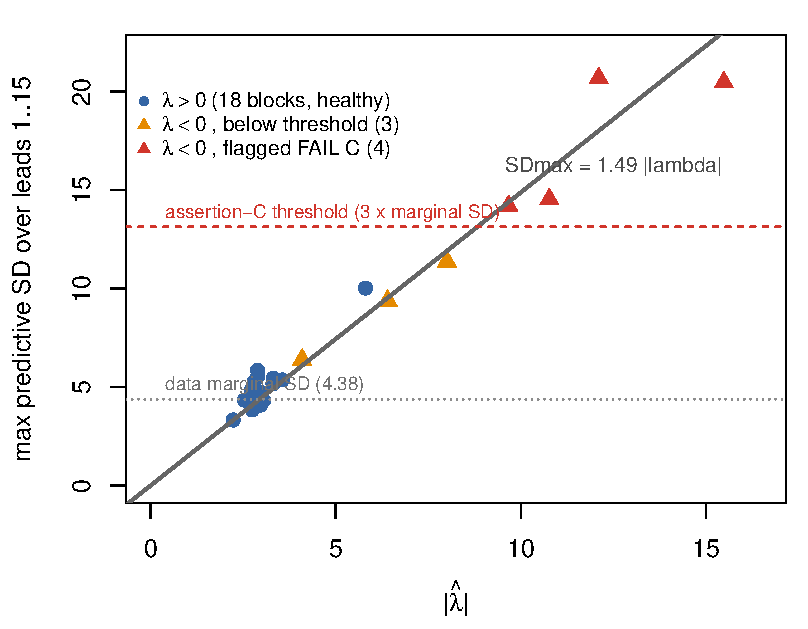
\includegraphics[width=0.72\textwidth]{sdmax_vs_lambda.pdf}
\caption{All $25$ refitted blocks. The maximum predictive SD over leads
$1$--$15$ is proportional to $|\hat\lambda|$: slope $1.49$, $R^2 = 0.987$
through the origin. Healthy fits ($\hat\lambda \approx 3$) and flagged
explosions ($|\hat\lambda| \approx 10$--$15$) lie on the same line; the
assertion-C threshold merely cuts the line at $|\hat\lambda| \approx 9$.
``Fixing the forecast'' is therefore not an available move: the forecast is a
faithful amplifier of $|\hat\lambda|$.}
\label{fig:law}
\end{figure}

\section{The ridge, exactly}

With one knot ($K = 1$) the observation equation at site $s$, time $t$ is
\begin{equation}
  y_{st} \;=\; x_{st}'\beta \;+\; \lambda\, z_t \;+\; \varepsilon_{st}/\sqrt{\tau_t},
  \qquad z_t \sim \hn(0, \tau_t^{-1/2}),
  \label{eq:model}
\end{equation}
so the likelihood involves $(\beta_0, \lambda, \{z_t\})$ \emph{only through}
\begin{equation}
  m_t \;=\; \beta_0 + \lambda z_t .
  \label{eq:mt}
\end{equation}
Fix any fitted trajectory $\{m_t\}$. Then for \emph{every} pair $(\beta_0^\ast,
\lambda^\ast)$ with $\lambda^\ast \ne 0$, the reassignment
\begin{equation}
  z_t^\ast \;=\; \frac{m_t - \beta_0^\ast}{\lambda^\ast}
  \label{eq:reassign}
\end{equation}
reproduces the data likelihood exactly, provided $z_t^\ast \ge 0$ for all $t$.
The likelihood is \emph{flat} on this two-parameter family. Identification
comes entirely from the prior structure on $z$: its half-normal marginal tied
to $\tau_t$, and the AR(2) Gaussian-copula dynamics on
$z^\star_t = \operatorname{hn.cop}(z_t, \tau_t^{-1/2})$.

Two branches of the family matter here.

\paragraph{The positive branch ($\lambda^\ast > 0$).} $z^\ast_t$ is an
increasing affine map of $m_t$; the $z$ path keeps the shape of the common
temporal signal. The prior is happiest near the truth, and $18$ of $25$ chains
sit there.

\paragraph{The reflected branch ($\lambda^\ast < 0$).} $z^\ast_t$ is a
\emph{decreasing} affine map of $m_t$: the latent path is flipped upside down,
and $\beta_0^\ast$ must exceed $\max_t m_t$ to keep $z^\ast_t \ge 0$ --- which
is exactly the observed $\hat\beta_0 \approx 26$--$35$ against a data mean of
$\approx 14.5$. Seven of $25$ chains ended here.

\section{Why the reflected branch is nearly free}

Three prices must be paid to sit on the reflected branch, and each one turns
out to be small.

\subsection{The prior on $\lambda$ charges almost nothing}

The prior is $\lambda \sim N(0, \code{lambda.s} = 20)$
(\code{mcmc\_ar2.R}). Whether $20$ is a standard deviation or a variance, the
log-prior difference between $\hat\lambda = -12$ and $\lambda = +3$ is a
fraction of a nat to a few nats --- negligible against a likelihood built from
$\text{ns} \times T$ observations that the branch reproduces \emph{exactly}.
A diffuse sign-symmetric prior cannot veto a sign flip that the likelihood
does not oppose.

\subsection{The half-normal marginal is satisfiable --- at the price of
smoothness}

On the reflected branch, by \eqref{eq:reassign},
\begin{equation}
  \bar{z^\ast} \;=\; \frac{\bar m - \beta_0^\ast}{\lambda^\ast},
  \qquad
  \sd_t(z^\ast) \;=\; \frac{\sd_t(m)}{|\lambda^\ast|} .
  \label{eq:shrink}
\end{equation}
The \emph{mean} constraint is easy: for any $\lambda^\ast$, choose
$\beta_0^\ast = \bar m - \lambda^\ast \bar z^{\,\text{target}}$ and the fitted
$\bar z$ lands wherever the half-normal marginal wants it ($\approx 1.5$ here).
This is precisely why \textbf{assertion A passes on every reflected fit}: the
marginal \emph{location} of $z$ is preserved by construction.

The \emph{temporal variation} is not. Equation~\eqref{eq:shrink} says the $z$
path's variation shrinks like $1/|\lambda^\ast|$: at $\hat\lambda = -12$ the
latent path has one-quarter of the temporal variation of the truth-branch path.
The model marginal $\hn(0, \tau^{-1/2})$ prescribes
$\sd(z) = \sigma\sqrt{1 - 2/\pi} \approx 1.1$; the reflected fit carries a $z$
path that is far too smooth for its own marginal. Note the asymmetry with the
\code{z.init} bug: there, the \emph{level} of $z$ was wrong ($7\times$ too
small) and A failed loudly; here the level is right and only the
\emph{second moment in time} is wrong --- a quantity assertion A never looks
at.

\subsection{The AR(2) copula absorbs the smoothness}

A too-smooth $z^\star$ path is not rejected by the AR(2) prior --- it is
\emph{fitted} by it, with a near-unit root. That is the observed
$\hat\phi_{1z} = 0.89$--$1.15$ (truth $0.80$; the joint stationarity constraint
keeps $\phi_1 + \phi_2 < 1$, so these are legal, highly persistent
configurations). The persistence in turn makes the smooth path likely, closing
the loop. This is the same self-reinforcing smoothness that appeared in the
\code{z.init} cascade, but running in the opposite causal direction: there,
frozen $z$ dragged $\phi_z$ to a unit root; here, inflated $|\lambda|$
\emph{requires} a smooth $z$, and the near-unit-root $\phi_z$ is what makes
smoothness cheap. $\phi_z$ is the accomplice, not the trigger.

Once inside, the chain is trapped: leaving the branch requires moving
$\lambda$ across zero \emph{and} dropping $\beta_0$ by $\approx 20$ \emph{and}
re-inverting the entire $z$ path simultaneously. Every one-coordinate Gibbs or
MH move away from the branch is individually catastrophic for the likelihood,
so the sampler stays. The posterior is bimodal; the chain picks a mode early
and cannot switch.

\section{Why the forecast explodes, quantitatively}

\code{forecast\_block} draws $z_{\text{fc}}$ from the model's own law: the
AR(2) recursion on the copula scale relaxes to $N(0,1)$, so $z_{\text{fc}}$
relaxes to its $\hn(0, \tau_{\text{fc}}^{-1/2})$ marginal with
\emph{full} temporal variance --- the forecast does not know the fitted path
was abnormally smooth. The skew channel then contributes spread
\begin{equation}
  \sd\!\big(\lambda\, z_{\text{fc}}\big)
  \;=\; |\lambda| \cdot \E[\sigma] \sqrt{1 - 2/\pi} \;\cdot\; (1 + \text{$\tau$-dispersion})
  \;\approx\; 1.13\,|\lambda| \;\text{at the floor},
\end{equation}
using $\E[\sigma] \approx 1.9$ from the fitted $(a, b)$. With the $\tau$
forecast's own dispersion and the residual noise folded in, the observed
constant is $1.49$ (Figure~\ref{fig:law}). At $\hat\lambda = 3$ this gives
$\approx 4.5$ --- climatology, as it must. At $\hat\lambda = -15.5$ it gives
$\approx 20$ against a data marginal of $4.38$ --- the residual explosions,
with nothing else needed to explain them.

The forecaster is again the detector, not the culprit: it is the only stage
that draws $z$ from the model law instead of reading the chain's smoothed
path, so it is the only stage where the branch's hidden inconsistency ---
inflated $|\lambda|$ against shrunken $z$ variation --- becomes visible.

\section{Two doors, one ridge}

\begin{center}
\begin{tabular}{p{0.30\textwidth}p{0.30\textwidth}p{0.30\textwidth}}
\toprule
 & \code{z.init} bug (fixed) & reflected branch (residual) \\
\midrule
entry & deterministic: every chain started at a $2.4\sigma$ tail point &
stochastic: $7/25$ chains drift in during burn-in \\
$\bar z$ (assertion A) & $7\times$ too small --- \textbf{fails} &
correct --- \textbf{passes} \\
what is wrong with $z$ & its level & its temporal variation \\
$\hat\lambda$ & $-56$ to $-98$ & $-4$ to $-15$ \\
$\hat\beta_0$ & $25$--$36$ & $19$--$35$ \\
$\hat\phi_{1z}$ & $\to$ unit root (effect) & $\to$ unit root (enabler) \\
predictive SD & $40$--$104$ & $6$--$21$, $= 1.49|\hat\lambda|$ \\
fix & delete one argument & none available at the code level:
this is the model's own geometry \\
\bottomrule
\end{tabular}
\end{center}

The common object is the ridge \eqref{eq:mt}. The \code{z.init} bug forced
every chain onto it through the $z$ coordinate; with that door closed, a
minority of chains still find it through the $(\lambda, \beta_0)$ coordinates.
The block-4 concentration ($3$ of the $4$ C-failures sit at seam $140$) has no
identified data-side cause --- dataset~4's own block~4 is perfectly healthy
($\hat\lambda = +2.97$) --- and is consistent with chance placement of $7$
stochastic events on a $5 \times 5$ grid, possibly tilted by whatever the
seam-$140$ prefix does to the early posterior on $\lambda$. We flag this
explicitly as unresolved rather than invent a mechanism for it.

\section{What can actually be done}

In rough order of cost:

\begin{enumerate}\itemsep3pt
  \item \textbf{Guard and reseed (pipeline-level, cheap).} The reflected branch
        is now detectable at fit time from three one-line symptoms: $\hat\lambda
        < 0$ (truth known in simulation), $\hat\beta_0$ far above the data mean,
        $\sd_t(\hat z)$ far below $\hat\sigma\sqrt{1 - 2/\pi}$. Refit flagged
        blocks with a different seed until clean. This is honest --- the
        assertion is a model-consistency check, not an outcome filter --- but it
        treats the symptom and would bias nothing only as long as the clean
        mode is the dominant one.
  \item \textbf{A new assertion A$'$ (diagnostic-level, cheap).} Assertion A
        checks the first moment of $z$; the reflected branch is invisible to it.
        Add A$'$: $\sd_t(\hat z_t) \approx \hat\sigma\sqrt{1-2/\pi}$, the
        \emph{second} temporal moment the model prescribes. Prediction, testable
        on the next diagnostic run: reflected fits violate A$'$ by roughly the
        factor $|\hat\lambda|/3$, healthy fits do not.
  \item \textbf{Break the sign symmetry in the prior (model-level, moderate).}
        In simulation the sign of $\lambda$ is known; even in applications the
        sign of skewness is usually known from the data (the backend itself
        initialises $\lambda$ at the sample skewness). A prior with mass on one
        side (e.g.\ $\lambda \sim \hn$, or $N(3, \text{small})$ in simulation)
        removes the reflected branch outright. This is the standard resolution
        of the same sign-reflection non-identifiability in skew-normal /
        factor-loading models.
  \item \textbf{Tighten \code{lambda.s} (model-level, blunt).} $N(0, 20)$
        charges a few nats at most for $|\lambda| = 12$. A scale chosen so that
        $|\lambda| \approx 12$ is genuinely expensive would starve the reflected
        branch without forbidding negative $\lambda$ --- but it also shrinks
        honest estimates, and picking the scale is a judgement call.
\end{enumerate}

Option 3 is the principled fix; options 1--2 are the immediate ones, require no
backend change, and are sufficient to produce the first trustworthy full
time-block study.

\section{The lesson this bug adds}

The \code{z.init} note ended by prescribing self-consistency assertions;
this episode is their first live test, and the verdict is double-edged.
Assertion A worked exactly as designed --- by \emph{passing}, it killed the
frozen-$z$ hypothesis on contact and forced the diagnosis toward the ridge.
Assertion C worked as designed --- it found every case worth finding, and
Figure~\ref{fig:law} shows it is a threshold on a clean underlying law rather
than an arbitrary flag. But the reflected branch slipped past A because A
checks the one moment of $z$ that the branch preserves \emph{by construction}.

\begin{quote}
An identifiability failure will satisfy every check that lies along the ridge.
Assertions must be chosen \emph{transverse} to the ridge: here, the level of
$z$ is along it, and the temporal variation of $z$ is across it.
\end{quote}

Concretely: a fit can reproduce the data mean, pass its own marginal-location
check, and carry legal AR coefficients, while being a reflection of the truth
with a four-fold inflated loading. The only quantities that betray it are the
ones the likelihood does not pin --- and those are exactly the quantities a
forecast consumes.

\end{document}
